% ------------------------------------
% Universidad de Costa Rica
% Facultad de Ingeniería
% Escuela de Ingeniería Eléctrica
% IE0499 - Proyecto Eléctrico
%
% PLANTILLA DEL TRABAJO ESCRITO
% ------------------------------------

% Tipo de documento
\documentclass[]{proyectoelectrico}

% A. PAQUETES Y MACROS ESPECIALES -------
% Aquellos que no están incluidos en la clase
% proyectoelectrico.cls

% -----------------------------------------
% OTROS PAQUETES E INSTRUCCIONES ESPECIALES
% -----------------------------------------

% Para insertar código fuente estilizado
\usepackage{listings}
	\lstset{basicstyle=\ttfamily,
    		breaklines=true,
            numbers=left, 
    		numberstyle=\tiny, 
    		stepnumber=1, 
    		numbersep=6pt}

% Para insertar símbolos extraños
\usepackage{marvosym}

% Para insertar texto fútil
\usepackage{lipsum}

% NUEVAS INSTRUCCIONES

\newcommand{\EIEx}{\textsc{Escuela \Lightning~ Ingeniería Eléctrica}}

% Definición de algunos símbolos matemáticos
\newcommand{\me}{\mathrm{e}}
\newcommand{\mi}{\mathrm{i}}
\newcommand{\mj}{\mathrm{j}}
\newcommand{\md}{\mathrm{d}}
\usepackage{libertine}
%\usepackage{libertinust1math}
\usepackage[T1]{fontenc}
\renewcommand*{\ttdefault}{cmtt}

% B. DATOS ------------------------------
% Todos los nombres incluyen dos apellidos
% y acentos y signos de puntuación apropiados.

% Título del proyecto
\titulo{Implementación de mapeo y localización simultánea para un robot móvil con ruedas mecanum.}

%% Autor (nombre y carné)
\autor{Stuart Leal Quesada}
\carne{B53777}

% Profesor(a) guía
\guia{Ing. Federico Ruíz Ugalde, Dr.rer.nat}

% Profesores lectores
\lectorA{Ing. Israel Arbaiza, Lic.}
\lectorB{Ing. Fabián Abarca Calderón, M.Sc.}

% Fecha de entrega del trabajo escrito
\mes{4}
\ano{2018}

% ------------------------------------

%%%%%%%%%%%%%%%%%%%
\begin{document}
%%%%%%%%%%%%%%%%%%%

\frontmatter

% 1. PORTADA
\portada

% 2. HOJA DE APROBACIÓN
\aprobacion

% 3. RESUMEN (EN ESPAÑOL E INGLÉS)
% --------------------------------
%% EL RESUMEN
% ----------

\begin{resumen}{palabras, claves, separadas, por, coma}

Este es el resumen del trabajo. Tiene un máximo de 300 palabras y debe ajustarse a una sola página en este formato.

\lipsum[1-2]

\end{resumen}
%% EL RESUMEN EN INGLÉS
% --------------------

\begin{theabstract}{Title of the Project in English}{keywords, separated, by, a, comma}

This is a test of the abstract of the project. It should not have more than 300 words or exceed one page in this template (whichever happens first).

\lipsum[1-2]

\end{theabstract}

% El entorno 'theabstract' tiene el formato \begin{theabstract}{A} ...B... \end{theabstract} donde A es el título del proyecto traducido de inglés a español y B es el contenido, en inglés, del resumen. Se recomienda buscar ayuda calificada para la elaboración y/o revisión de este resumen.

% 4. DEDICATORIA
%% LA DEDICATORIA
% --------------

\begin{dedicatoria}
Dedicado a
\end{dedicatoria}

% 5. AGRADECIMIENTOS
%% LOS AGRADECIMIENTOS
% -------------------

\begin{agradecimientos}

\lipsum[5]

\end{agradecimientos}

% 6. TABLAS DE CONTENIDO, FIGURAS Y TABLAS
% ----------------------------------------
\tableofcontents
\listoffigures
\listoftables

% 7. NOMENCLATURA
% ---------------
\input{contenido/nomenclatura.tex}

\mainmatter

% 8. CAPÍTULOS
% ------------
% ----------------------
  \chapter{Introducción}
% ----------------------
\label{C:introduccion}



%--------------------------------------------------------------------
Desde los años sesenta, con la revolución industrial, los humanos han sido relevados de operar tareas riesgosas. La tecnología ha evolucionado, siendo utilizada para realizar tareas más complejas, o de mucha precisión \cite{Garcia2007}. La fabricación de micro procesadores, o autos en masa son algunos ejemplos de productos que han florecido gracias a esta evolución.

Sin embargo, actualmente existen nuevas necesidades y mercados fuera de la tradicional manufactura. Por ejemplo, limpieza, cocina, construcción, agricultura, entre otras. Esto demanda una nueva generación de invenciones que puedan satisfacer estas necesidades \cite{Garcia2007}.

La robótica es la ciencia de percibir y manipular el mundo físico através de dispositivos mecánicos controlados por computadoras \cite{Thrun2005}. Hasta el día de hoy la robótica ha logrado perfeccionar los movimientos precisos milimétricamente, y las tareas repetitivas. Sin embargo, fuera de una línea de producción, estas ventajas no son útiles, pues por ejemplo en un hogar los ambientes son dinámicos y el robot por lo tanto debe poseer características cognitivas \cite{HelioAzevedoRenatoArcherITCenterandICM/USPJosePedroR.InstituteofMathematicalandComputerSciences2017}.

El laboratorio de investigación ARCOS-Lab (Autonomous Robots and Cognitive Systems) se enfoca primariamente en desarrollar e implementar nuevas técnicas en dispositivos mecánicos con el fin de satisfacer algunas de las necesidades mencionadas anteriormente.

Actualmente (2018) el ARCOS-Lab está trabajando en la construcción de un robot humanoide, el cuál se desea que pueda reconocer su ambiente, y realizar tareas dinámicas como cocinar. La navegación es uno de los aspectos más importantes que se debe desarrollar para cumplir el fin propuesto. Por lo tanto, el presente proyecto plantea implementar un algoritmo llamado SLAM (Simultaneous localization and mapping) en la navegación dos-dimensional de un robot omnidireccional con ruedas mecanum.

Una de las herramientas más potentes de hoy en día en el tema de la robótica es un sistema llamda ROS (Robot Operating System). El mismo se desarrolla primariamente en Linux, y posee muchas herramientas necesarias para realizar una tarea como la propuesta. El software ayuda a incorporar modularmente sensores y algoritmos de software desarrollados por científicos que trabajan en el área.

\newpage
\section{Alcance}
Se pretende implementar SLAM en robots pequeños denomindados ``\textit{mobile robots}'' dentro del contexto del ARCOS-Lab. Los mismos son plataformas de aproximadamente $50cm$ x $20cm$. Fueron contruidos para implementar los algoritmos de navegación, y realizar investigación en esta área, con el fin de perfeccionar el sistema que se utilizará para el robot humanoide. Las plataformas poseen en esencia el mismo sistema de ruedas omnidireccionales mecanum del robot humanoide.

En principio, es difícil experimentar con la base del robot humanoide desde un inicio. Primero está la limitación de que la misma plataforma está en un constante proceso de desarrollo, lo que quiere decir que se le hacen mejoras constantemente. Esto dificulta la disponibilidad de la base. Además, en los casos en que la plataforma se controle incorrectamente, los daños que pueda ocasionar a una persona o los objetos dentro del laboratorio son superiores a los que podrían ocasionar las plataformas más pequeñas.

\subsection{Equipo}
A continuación se hace una breve descripción del equipo principal utilizado para la construcción de las plataformas omnidireccionales utilizadas.

\begin{itemize}
\item \textit{Motores DC}: Los motores DC utilizados para cada una de las cuatro ruedas de la plataforma omnidireccional. Son motores de $12V$, con un consumo de aproximado $0.53A$ sin carga, y un codificador de cuadratura que produce 3415 pulsos por revolución. El motor logra alcanzar hasta 118rpm según la hoja de fabricante.
\item \textit{Roboclaw 2x15A}: Este controlador está diseñado para manejar dos motores DC de máximo 15A cada uno, por lo que se utilizarán dos de estos controladores para manejar los cuatro motores.
\item \textit{STM32F4}: Se necesita un controlador con capacidad de mandar los comandos de control hacia el Roboclaw para poder comandar la plataforma correctamente. Se utilizará un microcontrolador STM32F411-disco para esta tarea. La odemetría será calculada en este microcontrolador, en vez del Roboclaw para mayor precisión.
\item \textit{RaspBerry PI}: Se utiliza este microcontrolador, como la unidad de procesamiento principal en donde se controlarán los perifericos por medio del sistema de ROS. A esta tarjeta se conectará el Kinect y el Stm32F4.
\item \textit{Kinect 2}: Este será el sensor utilizado para la odometría visual. Será utilizado principalmente para generar la información del mapa, y posteriormente la ubicación del robot dentro del mismo mapa.
\end{itemize}

\subsection{Herramientas}
Se describen las herramientas que se utilizarán en el desarrollo del proyecto.

\begin{itemize}
\item \textit{ROS}: El desarollo e implentación de SLAM se realizará en ROS, puesto que es un sistema que permite la modularización de los diferentes componentes del robot. Facilita la conexión entre los diferentes perifericos. Posee librerías que contienen el código necesario para implementar SLAM.
\item \textit{Gazebo}: Un simulador de interacciones físicas para ROS, en donde se puede realizar la implementación completa del agoritmo de control para las plataformas móviles.
\end{itemize}

\subsection{Resultados}
El resultado final esperado es la implementación física del algoritmo a las plataformas ya existentes del laboratorio. Además, se realizarán simulaciones que muestren los resultados esperados en la realidad, esto con el fin de dividr en etapas la implementación, para facilitar la detección de errores. En otras palabras, se tendrá tanto la simulación como la implementación física del algoritmo de navegación autónoma.

\section{Justificación}
Este proyecto pretende brindar la base sobre la cuál nuevos proyectos pueden trabajar en nuevos algoritmos de navegación. Además, pretende fijar un primer paso para la implementación de navegación en el robot humanoide.

\section{Objetivos}

\subsection{Objetivo general}
Dotar a un robot omnidireccional con ruedas mecanum la capacidad de mapeo y localización simultánea.

\subsection{Objetivos específicos}
Para el desarrollo de este proyecto se establecieron los siguientes objetivos:

\begin{itemize} % lista con viñetas
    \item Desarrollar el software de control para los motores de las ruedas y los sensores de odometría.
    \item Desarrollar la infraestructura de comunicación entre el Raspberry Pi y el cuerpo del robot (motores y odometría). \item Implementar el software de comunicación y visualización del sensor de profundidad.
    \item Integrar todos los módulos del sistema (software y hardware) y realizar pruebas de conectividad y funcionamiento para cada módulo del sistema.
    \item Implementar el sistema de SLAM en la computadora principal.
    \item Determinar y ejecutar experimentos que permitan validar el funcionamiento completo de todo el sistema para realizar pruebas de mapeo y localización simultánea.
\end{itemize}

\section{Metodología}

\begin{enumerate}  %lista numerada
    \item Conectar el Kinect con una computadora corriendo Linux e utilizar ROS (Robot Operating System) para ver la imagen producida por la cámara.
    \item Convertir la imagen en formato PointCloud2 (3d) a un formato LaserScan (2d).
    \item Conectar el sensor láser Hokuyo a una computadora corriendo Linux e utilizar ROS para interpretar la imagen en formato LaserScan.
    \item Utilizar el simulador Gazebo en ROS con un modelo básico de un robot, e probar el uso de sensores y movimiento del mismo.
    \item Conectar el controlador de motores RoboClaw con un STM32F4 y hacer pruebas de comunicación.
    \item Diseñar el código necesario para leer el codificador de cuadratura que poseen los motores.
    \item Implementar el código necesario para la odometría de los motores.
    \item Diseñar un controlador PID para la velocidad del motor.
    \item Realizar pruebas de movimiento, e implemetar el protocolo de comunicación en el STM32f4.
    \item Utilizar un Joystick DualShock 4 en ROS y utilizarlo para mover el robot.
    \item Implementar el algoritmo de gmapping a el robot de la simulación en gazebo.
    \item Implementar el algoritmo de localización y navegación amcl en el simulador gazebo.
    \item Utilizar una Raspberry Pi para mandarle información de movimiento al STM32F4-Roboclaw. Mover los motores y hacer pruebas.
    \item Realizar el cálculo de odometría con el Raspberry Pi con la información dada por el RoboClaw.
    \item Confeccionar el módulo que conecta el STM32F4 con ROS.
    \item Trasladar lo implementado en Gazebo hacia el robot real.
    \item Realizar pruebas de funcionamiento, y corregir problemas.
\end{enumerate}

% ----------------------
\chapter{Nota teórica}
% ----------------------
\label{C:nota_teorica}

Un robot omnidireccional es una plataforma que se puede mover autónomamente. Son utilizadas en industrias de manufactura flexibles y en ambientes de servicio \cite{Batlle2009}. Hay tres aspectos importantes que posee un robot omnidireccinal. La figura \ref{F:omni} ayuda a ilustrar las tres características básicas de un rotot omnidireccional.

A continuación, se procede en las siguientes secciones a clarificar algunos conecptos necesarios para entender cómo se consiguen estas características en un robot móvil.

\begin{figure}[H]
    \centering
    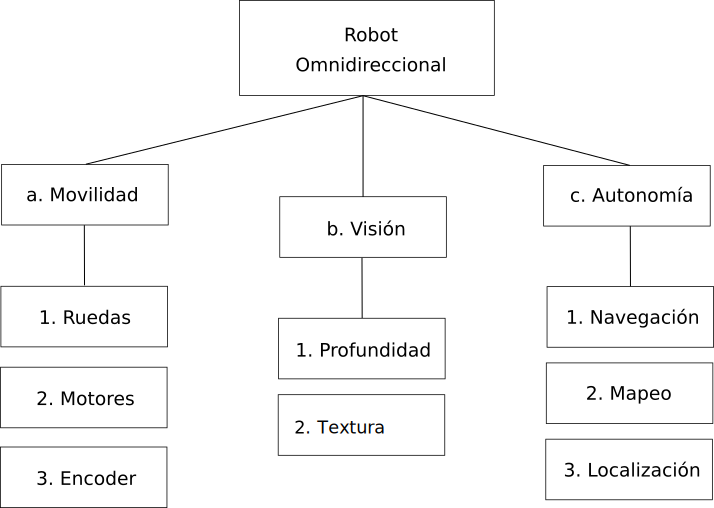
\includegraphics[scale=0.6]{imagenes/robot_omnidireccional.png}
    \caption{Diagrama de componentes de un robot omnidireccional. Autoría propia.}
    \label{F:omni}
\end{figure}


\section{Movilidad}
\subsection{Ruedas}
Existen varios aspectos a considerar cuando se diseña un robot: movilidad, control y posicionamiento. La primera hace referencia a la cantidad de movimientos que un robot puede realizar para llegar a una configuración final. Deben ser capaces de alcanzar cualquier posición y cualquier orientación en su plano de movimiento. Esto quiere decir que el marco del robot debe poseer tres coordenadas independientes del plano general de movimiento \cite{Batlle2009}.

El movimiento se puede realizar con un robot que tiene dos grados de libertad (se puede mover hacia adelante y atrás, con un ángulo de dirección), pero hay que maniobrar. Es más fácil realizar esta tarea si un robot tiene tres grados de libertad. Esto quiere decir, se puede mover hacia adelante y hacia atrás, izquierda derecha, y rotar. De esta manera, la movilidad aumenta, puesto que la cantidad de movimientos posibles que un robot puede realizar para llegar a una configuración final aumenta \cite{Batlle2009}.

Existe un tipo de ruedas, conocidas como ruedas omnidireccionales, que están compuestas de pequeños rodillos que habilitan el deslizamiento de la rueda en cierta dirección. En particular, las ruedas mecanum, como las que se muestran en la figura \ref{F:ruedas_mecanum}, son un caso especial de las ruedas omnidireccionales. Los rodillos están en cierto ángulo $\alpha$ de desface, que permite realizar los movimientos izquierda-derecha con una combinación de fuerzas específica para cada ruedas.

\begin{figure}[H]
  \centering
  \includegraphics[scale=0.3]{imagenes/ruedas_mecanum.png}
  \caption{Ruedas omnidireccionales Mecanum, con $\alpha = 45^\circ $. Tomado de \cite{Batlle2009}.}
  \label{F:ruedas_mecanum}
\end{figure}

La combinación de las diferentes velocidades en cada uno de los motores, producen los tres grados de libertad en el marco del robot. Específicamene, la kinemática del robot la define el autor \cite{Taheri2015}. A continuación, se muestran las ecuaciones que definen el movimiento del robot:

\begin{equation}
\begin{bmatrix}
w_1\\
w_2\\
w_3\\
w_4\\
\end{bmatrix}
= \frac{1}{r}
\begin{bmatrix}
1 & -1 & -(l_x + l_y) \\
1 & 1 & (l_x + l_y) \\
1 & 1 & -(l_x + l_y) \\
1 & -1 & (l_x + l_y) \\
\end{bmatrix}
\begin{bmatrix}
v_x \\
v_y \\
w_z \\
\end{bmatrix}
\label{E:kinematica_inversa}
\end{equation}

\begin{equation}
\begin{bmatrix}
v_x \\
v_y \\
w_z \\
\end{bmatrix}
= \frac{r}{4}
\begin{bmatrix}
1 & 1 & 1 & 1 \\
-1 & 1 & 1 & -1 \\
\frac{-1}{l_x + l_y} & \frac{1}{l_x + l_y} & \frac{-1}{l_x + l_y} & \frac{1}{l_x + l_y} \\
\end{bmatrix}
\begin{bmatrix}
w_1\\
w_2\\
w_3\\
w_4\\
\label{E:kinematica_directa}
\end{bmatrix}
\end{equation}

\begin{equation}
\begin{bmatrix}
\frac{d v_{x abs}}{dt} \\
\frac{d v_{y abs}}{dt} \\
\end{bmatrix}
 =
\begin{bmatrix}
cos(\frac{d w_z}{d t}) & -sin(\frac{d w_z}{d t}) \\
sin(\frac{d w_z}{d t}) & cos(\frac{d w_z}{d t}) \\
\end{bmatrix}
\begin{bmatrix}
\frac{d v_x}{dt} \\
\frac{d v_y}{dt} \\
\end{bmatrix}
\label{E:transformación}
\end{equation}

La ecuación \ref{E:kinematica_inversa} se utiliza para averiguar la velocidad necesaria en cada una de las ruedas, dado un comando de velocidad relativa al robot. Esto quiere decir que $v_x$ siempre es la velocidad del robot hacia adelante y hacia atrás, sin importar su posición con el mundo. $v_y$ siempre es la velocidad del robot hacia los lados, y lo mismo con $w_Z$.

La ecuación \ref{E:kinematica_directa} en conjunto con la ecuación \ref{E:transformación}, se utilizan para saber la posición real del robot en un plano x,y cartesiano. Es decir, se puede conocer la posición del robot en $x$, $y$, con respecto al mundo.

\subsection{Motores}
Para el robot omnidireccional en contrucción, se utilizarán motores DC. El diagrama básico de un motor DC se muestra en la figura \ref{F:motor_dc}.

\begin{figure}[H]
\centering
\includegraphics[scale=0.5]{imagenes/motor_dc.png}
\caption{Diagram simplificado de un motor DC. Tomado de \cite{Giblisco2016}}
\label{F:motor_dc}
\end{figure}

Cómo se observa en la figura, en un nivel básico, un motor DC posee dos o más embobinados, los cuáles ejercen una fuerza a un rotor el cuál posee un imán. Cuando pasa una corriente por el embobinado, la bobina produce un campo magnético, que produce una rotación en el rotor. Un comnutador causa que se entrege corriente en diferentes momentos hacia los diferentes embobinados, causando que el rotor gire constantemente \cite{Giblisco2016}.

Cabe destacar que esta conmutación se debe a una característica mecánica de la construcción del motor. Por lo tanto, lo único que se requiere para mover más rápido o más lento el motor, es más corriente o menos. Esto causará que el campo magnético producido sea mayor, y gire el rotor más velozmente.

\subsection{Encoder}
Un encoder es un dispositivo que se encuentra comunmente en sistemas de control modernos, y son utilizados para convertir desplazamiento lineal o rotacional en señales codificadas o pulsos de señal. Los encoders que publican información digital son conocidos como encoders absolutos \cite{Golnaraghi2017}.

Por otra parte, los encoders incrementales, producen un pulso en cada incremento, sin enmbargo no hacen distinción entre los incrementos \cite{Golnaraghi2017}.

En específico, un encoder de quadratura, posee dos sensores a un cierto desfase entre ellos, generalmente de $90^\circ$ . La figura \ref{F:encoder} muestra un ejemplo de un encoder utilizando un Hall Sensor. Este sensor es magnético, y produce la señal por una inducción que provoca el imán en dos sensores al girar.

\begin{figure}[H]
\centering
\includegraphics[scale=0.3]{imagenes/quad1.jpg}
\caption{Ejemplo de un encoder utilizando un Hall Sensor, y la señal producida por un encoder de cuadratura. Tomado de \cite{Golnaraghi2017}.}
\label{F:encoder}
\end{figure}

La señal que se produce, ayuda a identificar la dirección de rotación del motor, ya que el desfase entre las señales proporciona esta información. La frecuencia de los clicks, indican la velocidad del encoder, y finalmente, la cantidad de clicks ayudan a identificar la posición.

\section{Visión}
Para que un robot omnidireccional realice navegación, existe cierta información que resulta ser útil. Los sensores utilizados, generalmente permiten medir dos propiedades del ambiente: la profundidad de lo que se ve (La más importante), y el color de lo que se está viendo. La primera es esencial para lograr la navegación.

\subsection{Profundidad}
Existen muchos tipos de sensores diseñados para dar información de profundidad, como lo son sensores de ultrasonido, sensores laser de rango, entre otros. Sin embargo, la mayoría posee ciertas limitaciones que impiden el uso de los mismos en el campo de los robots autónomos, como lo son los problemas exactitud \cite{DanielMaierArminHornung2012}.

La llegada de los sensores de profundidad en 3D, como el Kinect o el Asus Xtion, que operan com patrones infrarojos han superado estas limitaciones. Estas cámaras son relativamente exactas, y proveen una información densa y tridimensional directamente del hardware \cite{DanielMaierArminHornung2012}. Por esta razón, los mismos sensores son muy utilizados en la navegación de robots autónomos.

Además de sensores como el Kinect, existen sensores de mayor precisión en un ámbito 2D, como lo son los sensores denominados en inglés \textit{Lidar}. Un ejemplo de estos sensores son producidos por la marca Hokuyo.

A continuación se muestra en la figura \ref{F:pointcloud} una muestra de la salida de un sensor de profundidad, utilizando una librería llamada PCL para visualizar la información.

\begin{figure}[H]
\centering
\includegraphics[scale=0.4]{imagenes/rviz_pointcloud.png}
\caption{Imagen de una captura de un sensor de profundidad. Tomado de \cite{Rusu2011}.}
\label{F:pointcloud}
\end{figure}

\subsection{Textura}

La textura en la parte de visión no es fundamental para realizar navegación. Esta información se puede utilizar para realizar detección de objetos, o encontrar cierto tipo de marcadores en el mundo para ubicarse mejor, sin embargo no es indispensable en el uso de navegación. Ejemplos de casos en donde se utilizan los sensores de color se pueden observar en \cite{Manduchi2005} y \cite{Lai2011}.


\section{Autonomía}

La autonomía en un robot, hace referencia a la capacidad del robot de comportarse de manera ``inteligente'' en algún aspecto \cite{Thrun2005}. Por ejemplo un vehículo que tenga la capacidad de manejarse sólo, y no provoque choques. Otro ejemplo sería robots que puedan limpiar un desastre nuclear, y no sean los humanos los que se vean expuestos a la radiación \cite{Thrun2005}.

Un robot que realice navegación autónomamente, se espera que pueda maniobrar en un espacio, ya sea nuevo o conocido, y pueda crear un mapa del lugar. La navegación por lo tanto, se compone de dos aspectos importantes. El primero, sería el mapeo y el segundo, la localización.

\subsection{Mapeo}

El objetivo del mapeo en un robot autónomo es aprender del entorno que rodea el robot, con el fin de realizar navegación en un futuro, o enviar este mapa a seres humanos. Es primordial tener un sistema robusto, para que los resultados del mapeo en diferentes ambientes sean consistentes.

Existen librerías que contienen la programación necesaria para realizar mapeo en un robot. Un ejemplo, es la librería denominada Navigation Stack, en el entorno de Ros. ROS (Robot Operating System), es un set de librerías, herramientas y convenciones que tratan de simplificar la tarea de crear comportamientos robóticos complejos y robustos a través de una amplia variedad de plataformas robóticas \cite{Quigley2009}.

La libreríad de ROS, posee un módulo llamado \textit{gmapping}, cómo parte del ``Navigation Stack''. De acuerdo con lo mencionado en \cite{Abbeel2006}, es un algoritmo que utiliza \textit{particle filter} (filtrado de partículas) de Rao-Blackwellized para realizar un mapeo a partir de sensores del tipo \textit{laser range}.

Esta solución ha probado ser muy eficiente, para ser utilizada en resolver el problema de mapeo y localización simultanea. El algoritmo utiliza un filtro de partículas, en el cuál cada partícula contiene un mapa individual del ambiente. Correspondientemente, la pregunta clave es cómo reducir la cantidad de partículas. El algoritmo en gmapping propone un acercamiento al problema que utiliza una distribución precisa que toma en cuenta no sólo el movimiento del robot, pero también la observación más reciente. Esto decrementa drásticamente la incertidumbre de la posición del robot, en el paso de la predicción del filtro \cite{Grisetti2007}. La figura \ref{F:mapa} muestra el ejemplo de un mapa generado por este módulo de ROS en el laboratorio de investigaciones de la Universidad de Texa.

\begin{figure}[H]
\centering
\includegraphics[scale=0.3]{imagenes/intel3d.jpg}
\caption{Mapa del edificio ACES en la universidad de Texas, cuarto piso. Tomado de \cite{Grisetti2007}.}
\label{F:mapa}
\end{figure}

De los mapas generados por Gmapping, las secciones grises son secciones desconocidas, o inexploradas. Las secciones en blanco son secciones bien conocidas que no posee obstáculos. Las secciones negras, son secciones que poseen obstáculos. La figura \ref{F:mapeando} muestra una visualización del proceso de mapeo en tiempo real, utilizando Rviz.

\begin{figure}[H]
\centering
\includegraphics[scale=0.4]{imagenes/map-gmapping.png}
\caption{Proceso de mapeo en tiempo real. Tomado de \cite{Grisetti2007}.}
\label{F:mapeando}
\end{figure}

\subsection{Localización}

El proceso de localización hace referencia a ubicar la posición del robot, relativa al mundo. Por lo tanto, se requiere de tener un mundo en el cuál localizarse. Este proceso se basa primariamente en la información de la odometría de las ruedas, tomado de lo que serían los encoders de los motores. La figura \ref{F:acml1} muestra un diagrama de este proceso. Sin embargo, siempre existe un pequeño nivel de error en la odometría, que puede ser causado por el deslizamiento, y otros problemas similares.

\begin{figure}[H]
\centering
\includegraphics[scale=0.4]{imagenes/diagrama_amcl.png}
\caption{Diagrama del proceso de localización utilizando únicamente la odometría de las ruedas. Tomado de \cite{ROSAMCL}.}
\label{F:acml1}
\end{figure}

Se debe por lo tanto utilizar alguna otra fuente de información para corregir los posibles deslizamientos que puede sufrir el robot, y tener una posición real del robot en el mundo. Existen varias formas de hacer esto, sin embargo el ``Navigation Stack'' utiliza un módulo llamado \textit{amcl}, para la localización.

\textit{Amcl} es un sistema de localización probablilística para un robot en movimiento de 2-D. Implementa el modelo adaptativo de localización Monte Carlo, como fué descrito por Dieter Fox, el cúal utiliza un filtro de partículas para llevar un record de la posición del robot contra un mapa conocido. La figura \ref{F:amcl} muestra el proceso de localización, utilizando la información de los nodos activos en ROS.

\begin{figure}[H]
\centering
\includegraphics[scale=0.4]{imagenes/mapa_amcl.png}
\caption{Diagrama del proceso de estimación de la posición realizado por ACML. Tomade de \cite{ROSAMCL}.}
\label{F:amcl}
\end{figure}

En otras palabras, AMCL trata de relacionar los \textit{laser scans} con el mapa, y así detecta si ha ocurrido alguna desviación  en la estimación de la pose basado en la odometría. Este ``deslizamiento'' es compensado publicando una transformación entre el marco del mapa, y el marco de la odometría, tal que el final la transformación del mapa hacia la base corresponda con la posición real del robot en el mundo.


\subsection{Navegación}

Para empezar a diseñar el aspecto de la navegación en un robot, se deben tener principalmente dos cosas. La primera que el robot se pueda mover inteligentemente, y maniobrar lo menos posible. Por lo tanto, un robot que posea tres grados de libertad es deseable, pues hace que la tarea de desplazarse en un ambiente sea bastante sencilla \cite{Batlle2009}.

Además se necesita saber la distancia que ha recorrido el robot en su plano, y cuánto ha rotado. Esto para que el robot sepa que el cambio en la información del sensor de profundidad se debe a un cambio en su posición, y no a un cambio en el mundo. Esto se logra a través de los encoders que se encuentran en los motores del robot.

Finalmente, se necesita un sensor de profundidad, como se habló anteriormente. Esto le permitirá al robot descubrir su entorno, y crear un mapa del mismo.

Igual que para el caso del mapeo, la librería de Navigation Stack en ROS continen la programación necesaria para realizar navegación, siempre y cuando el robot cumpla con las características anteriormente descritas.

El Stack de Navegación de ROS requiere dos mapas de costos, uno local y otro global, los cuáles contienen la información que representa la proyección de obstáculos in un plano 2D, así como un un radio de seguridad, donde se garantíza que el robot no colisionará con ningún otro objeto, sin importar su orientación \cite{Longhi}.

La navegación se realiza utilizando un módulo llamado \textit{global\_planner}, el cúal utiliza un mapa actual, y el radio del robot para planear una ruta del punto A al punto B.

\begin{figure}[H]
\centering
\includegraphics[scale=0.5]{imagenes/globalplanner.png}
\caption{Ejemplo de un uso del global planner en ROS, para obtener una posible ruta. Tomado de \cite{ROSPLANNER}.}
\end{figure}

Este módulo utiliza diferentes algoritmos, que pueden ser activados o desactivados para realizar la planeación de las rutas, como el algoritmo Dijkstra's.

% --------------------
  \chapter{Diseño}
% --------------------
\label{C:diseño}

Para la etapa de diseño, se dividirá en tres partes. La primera, será el diseño eléctrico del carrito omnidireccional, con los componentes necesarios para funcionar. La segunda es el diseño del código para el carrito omnidireccional, encargado del control de los motores y la odometría de las ruedas. Por último, se hablará del diseño necesario del lado de la computadora principal, para lograr la navegación y el mapeo.

\newpage

\subsection{Carrito omnidireccional}
Para la primera etapa, se utilizará el esquema básico presentado en la figura \ref{F:diagrama}. Se requiere de un sistema que pueda controlar los motores, y además llevar control de la odometría de las ruedas. Además se deberá incorporar el sensor de profundidad en el carrito omnidireccional.

\begin{figure}[H]
\centering
\includegraphics[scale=0.6]{imagenes/diagrama_diseno.png}
\caption{Diagrama básico de la implementación de la parte elétrica del carrito omnidireccional. Autoría propia.}
\label{F:diagrama}
\end{figure}

Empezando por los \textbf{motores}, se utilizarán motores DC Actobotics 638276. La hoja de fabricante con los datos en la sección de los apéndices. Además, en la tabla \ref{T:actobotics} se muestra la información más relevante de los motores a utilizar, como por ejemplo el consumo máximo, la tensión de trabajo, y la relación de los engranes.

\begin{table}[H]
\caption{Información más relevante de los motores Actobotics, a ser utilizados. Autoría propia.}
\begin{tabular}{|l|l|}
\hline
Especificación                & Valor         \\ \hline
Voltage de operación          & 6-12 VDC      \\ \hline
Corriente máxima de operación & 0.53 A        \\ \hline
Velocidad máxima sin carga    & 118 $\pm$ 12 rpm \\ \hline
Corriente máxima detenido     & 20 A          \\ \hline
Razón de los engranes         & 1/71          \\ \hline
Clicks del encoder por revolución & 3408      \\ \hline
\end{tabular}
\label{T:actobotics}
\end{table}

Se utilizarán cuatro motores, uno para cada rueda, conectados a ruedas mecanum genericas, de 6mm de diámetro. Estas son ruedas omnidireccionales con rodillos a un ángulo de $\alpha = 45^\circ$.

En lo que concierne a los \textbf{controladores} de los motores, no se diseñarán, puesto que se utilizarán controladores comerciales de marca IonMotion Roboclaw. En específico, se utilizará el modelo Roboclaw 2x15A. En el cuadro \ref{T:roboclaw} se resumen los datos más importantes de este controlador.

\begin{table}[H]
\caption{Información más relevante de los controladores Roboclaw 2x15A. Autoría propia.}
\begin{tabular}{|l|l|}
\hline
Especificación                      & Valor          \\ \hline
Tensión de la batería principal     & 6-34 VDC       \\ \hline
Tensión de la batería lógica        & 6-34 VDC       \\ \hline
Bits de los contadores para encoder & 32 bits        \\ \hline
Velocidad máxima sin carga          & 118 +- 12 rpm  \\ \hline
R232 Baud Rate                      & 460,800 Bits/s \\ \hline
Tensión de I/O                      & 3.3 VDC        \\ \hline
\end{tabular}
\label{T:roboclaw}
\end{table}

Es importante mencionar, que estos controladores se utilizan para manejar los motores. Pueden manejar hasta dos motores, y son muy versátiles en cuánto a cómo se pueden utilizar. En particular, para este proyecto se usará la comunicación serial que posee el controlador. En la figura \ref{F:roboclaw} se muestran los pines que posee el roboclaw. En específico, los pines S1, y S2 se pueden utilizar como puertos USART para comunicación serial. La tabla \ref{T:pines} muestra las funcionalidades que pueden cumplir cada pin.

\begin{figure}[H]
\centering
\includegraphics[scale=0.5]{imagenes/roboclaw.png}
\caption{Muestra de los pines de un Roboclaw 2x15A fabricado por IonMotion. Tomado del manual del fabricante.}
\label{F:roboclaw}
\end{figure}

\begin{table}[H]
\centering
\caption{Tabla con las funciones de los pines en un Roboclaw 2x15A fabricado por IonMotion. Tomado del manual del fabricante.}
\includegraphics[scale=0.7]{imagenes/pines.png}
\label{T:pines}
\end{table}

Se utilizará una frecuencia de 115200 en la transmisión serial, ya que es la más alta soportada por el dispositivo. En el modo llamado ``Packet Serial'', el cuál funciona mediante el protocolo RS-232 para controlar la dirección y velocidad de cada uno de los motores.

El fabricante da ejemplo de código que se puede utilizar para enviar comandos, y especifica el protocola utilizado en el manual de usuario. Todas las instrucciones utilizan un checksum crc16bit para verificación de las intrucciones.

Siguiendo el esquema de la figura \ref{F:diagrama}, los controladores Roboclaw van conectados al \textbf{microcontrolador} STM32F411. La principal función de este microcontrolador será llevar cuenta de la odometría de cada una de las ruedas, y del robot como tal. Además, este aceptará instrucciones por USB del Raspberry Pi, de movimiento en el formato $(V_X, V_Y, W_Z)$ y enviará información de vuelta de la odometría del robot en el formato $(X_X, X_Y, \alpha_Z)$. También enviará instrucciones de movimiento a los dos controladores Roboclaw, y controlará la velocidad de cada motor por medio de un PID, en lazo cerrado con la información del encoder como entrada.

El esquema mostrado en la figura \ref{F:diagrama_stm} muestra en resumen lo que se explicó anteriormente.

\begin{figure}[H]
\centering
\includegraphics[scale=0.5]{imagenes/microcontrolador_diagrama.png}
\caption{Diagrama de las funciones que debe realizar el microcontrolado STM32F411. Autoría propia.}
\label{F:diagrama_stm}
\end{figure}

Es importante notar, que la programación del microcontrolador se realizará mediante las liberías libopencm3 y libopencm3-plus, las cuáles permiten escribir el código en el lenguaje de programación C. Además, el microcontrolador posee las funciones para leer los encoders directamente, puesto que posee timers que se pueden configurar en un modo para leer codificadores de cuadratura.

Información sobre el uso de encoders de cuadratura en el stm se puede encontrar en apéndice correspondiente.

Finalmente, un diagrama de las conexiones eléctricas se puede encontrar en la figura \ref{F:conexiones}. En este diagrama se incluye la información de los pines pertinentes en cada dispositivo.

\begin{figure}[H]
\centering
\includegraphics[scale=0.63]{imagenes/diagrama_electrico.png}
\caption{Diagrama de las conexiones eléctricas entre los dispositivos. Autoría propia.}
\label{F:conexiones}
\end{figure}

\subsection{Código}




\newpage

El capítulo 3 y los subsiguientes (si fueran necesarios), mostrarán el trabajo realizado en el proyecto, por lo que su cantidad, títulos y divisiones, se dejan a discreción del estudiante, con la aprobación del profesor guía y demás miembros de Tribunal evaluador.

Estos capítulos muestran el ``producto'' del trabajo realizado en el proyecto, por lo cual constituyen la parte medular del informe. Debe explicarse en forma clara, qué se hizo, cómo se hizo y qué se obtuvo.

Cuando se agregan o remueven del texto elementos que aparecen en los índices (general, de figuras, de cuadros) que están en el preámbulo del informe, así como cuando se agregan o remueven citas a las fuentes bibliográficas, que aparecen en la Bibliografía al final del documento, es necesario ejecutar dos o tres veces la compilación del documento, para que estas listas se confeccionen nuevamente y se muestren correctamente.  También, en el caso de agregar o quitar ecuaciones, es necesario recompilar dos o tres veces el documento, para que se renumeren las ecuaciones y  las referencias a estas.

\begin{equation}
x_{1,2} = \frac{-b \pm \sqrt{b^2 - 4ac}}{2a}
\end{equation}

\section{Manejo de las fuentes bibliográficas}
Cuando se realiza un trabajo de desarrollo o investigación, siempre se parte del trabajo realizado por otras personas. Es por lo tanto indispensable, hacer referencia a las fuentes bibliográficas (referencias) utilizadas.

En \LaTeX se utiliza BibTeX para el manejo de la bibliografía.  La información de las fuentes consultadas (libros, artículos de revista o ponencias en congresos, tesis, etc.), se almacenan en un archivo \texttt{.bib} (base de datos de las fuentes bibiográficas), sin preocuparse del formato en que estas serán mostradas en el informe.  Para la creación y manejo de este archivo, se puede utilizar el programa JabRef\footnote{http://jabref.sourceforge.net/} o uno similar.

La forma en que las fuentes son listadas en el apartado Bibliografía, y como son mostradas en el texto cuando se citan, depende del \emph{estilo} seleccionado para esto.

\begin{equation}
Z = \begin{cases}
\sqrt{\epsilon_r - \cos^2 \theta}/\epsilon_r & \text{para polarización vertical} \\
\sqrt{\epsilon_r - \cos^2 \theta} & \text{para polarización horizontal} \\
\end{cases}
\end{equation}

Para el informe del proyecto eléctrico, se debe utilizar el formato APA\footnote{American Psychological Association, http://www.apa.org/}.  En inglés, este se establece utilizando el estilo \texttt{apalike}.

\begin{equation}
 e^{jx} = \cos{x} + j \sin{x}
\end{equation}

Junto con la clase \texttt{eieproyecto} se suministra el archivo de estilo de bibliografía \texttt{apalike\_es.bst}, en el cual se han cambiado los términos en ingles (ej. ``and'', ``In'', Edition y otros) por su equivalente en español.  Este archivo debe colocarse en la misma carpeta, en donde están los demás archivos utilizados para la confección del informe.

\begin{equation}
\int_0^\infty e^{-x^2} \mathrm{d}x = \frac{\sqrt{\pi}}{2}
\end{equation}

\begin{equation}
\mathbb{A-Z} \quad
\mathcal{A-Z}
\end{equation}

Por lo tanto, la lista de las fuentes bibliográficas utilizadas se confecciona automáticamente, a partir de las citas hechas en el texto.  Solo las fuentes citadas aparecerán en la bibliografía.

\begin{equation}
u(x) =
  \begin{cases}
   \exp{x} & \text{si } x \geq 0 \\
   1       & \text{si } x < 0
  \end{cases}
\end{equation}

Como se indicó anteriormente, se emplean \texttt{cite} y \texttt{citep} para hacer las citas.  Cual de estos dos comandos conviene utilizar, dependerá del contexto en que se haga la cita.  Según la redacción del párrafo, puede convenir que la fuente se indique en el formato ``Autor (año)'', pero en otros casos pudiera ser preferible que esta aparezca en el formato ``(Autor, año)''.

\begin{equation}
r(t) = \Re \left\lbrace \frac{\lambda}{4\pi} \left[ \frac{\sqrt{G_0} u(t) e^{-j2\pi r_0/\lambda}}{r_0} + \frac{\Gamma \sqrt{G_1} u(t-\tau) e^{-j2\pi r_1/\lambda}}{r_1} \right] e^{j2\pi f_c t}  \right\rbrace
\end{equation}

%% --------------------------------
  \chapter{Sobre el uso de \LaTeX}
% --------------------------------
\label{C:sobre_LaTeX}

\section{Introducción}

\LaTeX~ es un editor de texto bajo el paradigma de edición de texto ``lo que ve es lo que quiere decir'' (WYSIWYM, del inglés \emph{What You See Is What You Mean}) en el que se utiliza un lenguaje de descripción de formato\footnote{En ese sentido parecido al HTML}. Este paradigma es diferente a su contraparte y tradicional paradigma WYSIWYG (del inglés \emph{What You See Is What You Get}, ``lo que ve es lo que obtiene''), en el que se edita el texto y los demás elementos en una interfaz gráfica. Este es el caso de herramientas de ofimática como Microsoft Office, OpenOffice y LibreOffice y editores gráficos de todo tipo.

\begin{quote}
\LaTeX~ ``...es un sistema de composición lógica, por oposición a los sistemas de composición visual o programas WYSIWYG (\ldots) Con el sistema \LaTeX, lo que el autor escribe y ve en la pantalla del ordenador es el contenido del documento y su estructura lógica, pero entre estos y el documento compuesto hay un paso intermedio de procesamiento o \emph{compilación} del documento mediante el sistema \LaTeX'' \cite{Valiente2001}.
\end{quote}

Existe bibliografía extensa (incluyendo \cite{Valiente2001}\cite{Gratzer2001}\cite{Krishnan2003}\cite{Oetiker2014}\cite{Wikibooks2016}) donde se puede ampliar sobre \LaTeX. Así mismo, en Internet hay gran cantidad de tutoriales, comunidades y foros sobre el tema, como en \cite{StackExchange2016}. Se recomienda consultar estas fuentes para ampliar las posibilidades de escritura con este lenguaje.

En este capítulo se incluyen y explican algunos de los elementos básicos y más utilizados para la redacción en \LaTeX: ecuaciones, figuras, tablas, además de referencias a bibliografías, secciones, entre otras cosas, y puede ser utilizado como base para la elaboración del trabajo escrito del curso.

\subsection{¿Por qué \LaTeX? (opcional)}

\LaTeX~ es un paradigma de edición de texto utilizado ampliamente en la comunidad científica y tecnológica de todo el mundo, en publicaciones, revistas, libros y más. 

Tiene la virtud de facilitar la composición de un documento bien diseñado que ahorra toda la cuestión de forma para el editor.

La siguiente lista\footnote{Adaptado de \url{http://haptonstahl.org/latex/whyuse.php}} explica algunos puntos acerca del uso de \LaTeX.

\begin{description}

\item[Documentos estructurados] 
Es más fácil crear documentos estructurados en \LaTeX~ que en Word u otros editores. Un documento estructurado es un \emph{paper}, artículo, libro o tesis con capítulos, secciones, subsecciones, apéndices, tablas de contenidos, índices, etc. Los capítulos y secciones usualmente son enumerados secuencialmente, están listados en una tabla de contenidos, etc. Cuando se hacen cambios, todas las referencias relativas tienen que ser actualizadas. Todo esto es trivialmente fácil en \LaTeX.

Si no se quiere pensar acerca del formato y solo se quiere que el \emph{software} haga las cosas verse bien, hay que usar \LaTeX.

\item[Ecuaciones] 
Es más fácil y rápido escribir símbolos matemáticos utilizando \LaTeX~ que con MS Word. Una o dos páginas de fórmulas probablamente harán caer MS Word. Cientos de páginas de fórmulas no harán caer a \LaTeX.

\item[Calidad de tipografía e impresión] 
La escritura en \LaTeX~ es superior a la de otros procesadores de texto. Más referencias sobre esto en \url{http://nitens.org/taraborelli/latex}.

\end{description}

%%%%%%%%%%%%%%%%%%%%%%%%%%%%%%%%%%%%%%%%%%%%%%
\section{Las partes de un documento de \LaTeX}
%%%%%%%%%%%%%%%%%%%%%%%%%%%%%%%%%%%%%%%%%%%%%%

\subsection{Preámbulo y cuerpo del documento}
%%%%%%%%%%%%%%%%%%%%%%%%%%%%%%%%%%%%%%%%%%%%%

Los archivos \texttt{.tex} de donde se generan los documentos en \LaTeX~ tienen dos grandes secciones: el encabezado o preámbulo y el cuerpo del documento.

En el \textbf{encabezado} del documento se definen los parámetros más importantes del documento, y se invocan los ``paquetes'' que permiten la edición de características especiales. Entre las características que se pueden definir aquí están: tamaño del papel, tamaño y tipo de tipografía, tipo de documento (reporte, artículo, libro, carta\ldots), numeración, autor, fecha, título y más. 

Además de estas definiciones generales, se deben cargar todos los \textbf{paquetes} que permiten hacer ediciones especiales como: introducir hipervínculos, agregar colores, agregar imágenes, editar encabezados y pies de página, etc. 

Para utilizar un paquete se escribe la instrucción \verb+\usepackage[opciones]{nombredelpaquete}+, donde las opciones están definidas por cada paquete particular. 

Por ejemplo \verb+\usepackage[spanish]{babel}+. El paquete Babel permite cambiar la lengua del documento (en inglés por defecto), y entre paréntesis cuadrado se especifica que sea español.

Los paquetes que utiliza \LaTeX~ están en un repositorio (ver Sección \ref{S:programas}). La documentación de los paquetes puede encontrarse en la página de CTAN (\textit{Comprehensive TEX Archive Network}), \url{https://www.ctan.org/}.

Uno de los elementos más importantes de \LaTeX~ es el \emph{entorno}. Un entorno (\emph{environment}) siempre inicia con \verb+\begin{nombredelentorno}+ y finaliza con \verb+\end{nombredelentorno}+. Dentro de él, todo el contenido va a tener un formato característico dependiendo del tipo de entorno. Las ecuaciones, figuras y tablas tienen su propio entorno. Hay otros para listas numeradas, resumen, teoremas, texto centrado\ y más. El mismo cuerpo del documento es un gran entorno \texttt{document}.

A continuación se describirá el uso de algunos de los entornos más importantes: ecuaciones, tablas y figuras.

\subsection{Ecuaciones}
%%%%%%%%%%%%%%%%%%%%%%%

Hay tres tipos de ecuaciones posibles: unas en línea, o dentro del párrafo, otras en modo \emph{display} con numeración y sin numeración. 

\begin{description}

\item [Las ecuaciones en línea] están rodeadas por los símbolos \verb+$ $+ (una forma abreviada de crear el entorno). Se utilizan cuando se coloca una fórmula en un párrafo, por ejemplo $ {{B}_{f}}\ge 0,2 $, que no lleva numeración y que debe estar alineada con el texto. \LaTeX~ se encargará de ajustar su tamaño y ubicación, como cuando se introduce una raíz cuadrada $ \sqrt {{b^2} - 4ac} $ o una integral  $ \int_0^\infty e^{-x}\,\mathrm{d}x $. 

\item [Las ecuaciones numeradas] se hacen dentro del entorno \texttt{equation}. Ejemplos de ecuaciones se muestran a continuación.

\begin{verbatim}
\begin{equation}
x_{1,2} = \frac{-b \pm \sqrt{b^2 - 4ac}}{2a}
\end{equation}
\end{verbatim}

\begin{equation}
x_{1,2} = \frac{-b \pm \sqrt{b^2 - 4ac}}{2a}
\end{equation}

\begin{equation}\label{E:desigualdad}
{B}_{f}\ge 0,2
\end{equation}

\begin{equation}\label{E:anchodebanda}
BW\ge 500\text{ MHz}
\end{equation}

donde $ {B}_{f} $ es el ancho de banda fraccional y se define como:

\begin{equation}\label{E:fraccional}
{{B}_{f}}=\frac{BW}{{{f}_{c}}}=\frac{\left( {{f}_{H}}-{{f}_{L}} \right)}{{\left( {{f}_{H}}+{{f}_{L}} \right)}/{2}\;}
\end{equation}

donde $f_H$ y $f_L$ son las frecuencias superior e inferior de la banda de transmisión de -10 dB, $ BW $ es el ancho de banda y $f_c$ la frecuencia central.

El estilo de la numeración depende del tipo de documento (\texttt{article}, \texttt{report}, \texttt{book}\ldots) y obedecerá (si no se especifica lo contrario) la secuencia numérica.

\item [La ecuaciones no numeradas] se deben utilizar en ocasiones, sobre todo cuando se trata de pasos intermedios o cálculos y no la deducción de alguna expresión. Para ello se deben utilizar los símbolos \verb+\[+ y \verb+\]+ (otra forma abreviada de crear el entorno) para rodear la ecuación.

\[
 \lim_{x \to \infty} \exp(-x) = 0
\]

\[
 R_{pu} = 2,7~\si{\kilo\ohm}
\]

\end{description}

Será necesario también en ocasiones incluir texto dentro de las ecuaciones. Pero es necesario escribir este texto dentro de los comandos \verb+\text{}+, \verb+\textbf{}+ o similares, para que se les aplique el espaciado y formato correctos. De otro modo sucede lo que se muestra en la ecuación (\ref{E:sintexto}), mientras que la ecuación (\ref{E:contexto}) muestra el uso corregido, incluyendo cierto formato añadido para resaltar.

\begin{equation}\label{E:sintexto}
Ciclo de trabajo = \frac{Tiempo en alto}{Per\acute{i}odo}
\end{equation}

\begin{equation}\label{E:contexto}
\text{Ciclo de trabajo} = \frac{\textsf{Tiempo en alto}}{\textbf{Per\'{i}odo}}
\end{equation}

A pesar de que la escritura de ecuaciones directamente en \LaTeX~ puede resultar algo complicada al principio, basta con una rápida investigación en la vasta información de las referencias suministradas y en la red\footnote{Hay muchas comunidades de usuarios en internet en foros y demás que resuelven estos problemas típicos} para encontrar la forma de realizar la ecuación deseada. Como alternativa, se puede utilizar un editor gráfico de ecuaciones como \href{http://www.dessci.com/en/products/mathtype/}{MathType} y de ahí exportar a \LaTeX\footnote{Para hacerlo: en la ventana de edición de ecuaciones de MathType se debe ir a \textsf{Preferences / Cut and Copy Preferences}, en la ventana emergente se debe seleccionar la opción \textsf{MathML or TeX} y en la lista desplegable escoger \textsf{LaTeX 2.09 and later}. En la misma ventana de edición se selecciona y copia la ecuación. La barra de estado mostrará: \textsf{Translated (LaTeX 2.09 and later)}.}. Es necesario, aún así, aprender los comandos básicos que facilitan y hacen más rápida la composición de fórmulas.

También se pueden editar ecuaciones en la aplicación en internet disponible en \url{http://rinconmatematico.com/latexrender/} en la cual se puede ver el resultado de la ecuación editada.

\subsection{Figuras}\label{S:Figuras}
%%%%%%%%%%%%%%%%%%%%%%%%%%%%%%%%%%%%%

Para las figuras existe un entorno llamado \verb+figure+, dentro del cual se ubican y configuran las imágenes.

Para ``llamar'' al archivo se debe hacer una referencia a su ubicación. Si está ubicada en la misma carpeta del documento se escribe \verb+nombre_de_la_imagen.jpg+\footnote{O cualquier formato de imágenes soportado, como .png, .gif y otros}. Pero los archivos de imágenes, de preferencia y por una cuestión de orden, deben colocarse dentro de una carpeta dedicada. Entonces, si está dentro de una carpeta se indica \verb+./carpeta/nombre_de_la_imagen.jpg+. Para subir un nivel en las carpetas se utiliza \verb+../carpeta/subcarpeta/nombre_de_la_imagen.jpg+. 

La imagen ``Nube de tormenta con rayos y lluvia'' es un ejemplo de imagen insertada.

\begin{figure}[H]
\centering
\includegraphics[width=0.2\textwidth]{./imagenes/tormenta.png} 
\caption{Nube de tormenta con rayos y lluvia}
\label{F:tormenta}
\end{figure}

La instrucción para insertar la gráfica es:


\begin{lstlisting}[]
\begin{figure}[H]
\centering
\includegraphics[width=0.2\textwidth]{./imagenes/tormenta.png} 
\caption{Nube de tormenta con rayos y lluvia}
\label{F:tormenta}
\end{figure}
\end{lstlisting}

La descripción es la siguiente:

\begin{itemize}\itemsep0pt \parskip0pt \parsep0pt
\item \verb+\begin{figure}[H]+ en la línea 1 inicia el entorno de la figura y declara que será ubicada inmediatamente luego del texto, con \verb+[H]+.
\item \verb+\centering+ en la línea 2 es una instrucción abreviada para indicar que la figura estará centrada.
\item \verb+\includegraphics[width=0.2\textwidth]{./imagenes/tormenta.png}+ es la instrucción para insertar el archivo de la imagen, junto con indicaciones adicionales sobre el tamaño (un 20 \% del ancho del texto).
\item \verb+\caption{Nube de tormenta con rayos y lluvia}+ la instrucción  \texttt{caption}\footnote{En inglés, es bastante explícita esta instrucción, y en general puede decirse lo mismo de todos los comandos de \LaTeX, (ver por ejemplo \textsf{footnote}, \textsf{includegraphics}, \textsf{subsection}, etc.)} es el pie de figura con el nombre y la explicación. El número de figura lo inserta \LaTeX~ automáticamente.
\item \verb+\label{F:tormenta}+ es una etiqueta para referencia dentro de otras partes del texto.
\item \verb+\end{figure}+ cierra el entorno de la figura.
\end{itemize}

Como buena práctica, se recomienda nombrar el archivo de la imagen igual que la etiqueta, y con \textit{un nombre representativo}. Los nombres no deben tener espacios ni tildes ni eñes. Por ejemplo: \verb+senal_entrada_sinusoidal.jpg+.

\LaTeX, por defecto, va a ubicar las imágenes arriba o debajo de la página, y no inmediatamente después del texto en el que se escribe dentro del código, excepto que se indique lo contrario con \verb+\begin{figure}[h!]+ o con \verb+\begin{table}[H]+ utilizando el paquete \verb+float+.

Adicionalmente, se puede ubicar varias imágenes dentro de un mismo entorno de figura, como en la Figura \ref{F:subfiguras}. Ahí se muestran cuatro figuras distintas dentro del mismo entorno, donde se puede hacer referencia al transistor en \ref{F:subfig1}, al LED en \ref{F:subfig2}, al fotoconductor en \ref{F:subfig3} y al circuito integrado en \ref{F:subfig4}.

\begin{figure}[h!]
\centering
\subfloat[Transistor (texto que aparece en el índice)][Transistor en encapsulado TO-220]{
	\includegraphics[width=0.2\textwidth]{./imagenes/transistor.jpg}
	\label{F:subfig1}}
\qquad
\subfloat[LED][LED blanco de baja potencia]{
	\includegraphics[width=0.2\textwidth]{./imagenes/led.jpg}
	\label{F:subfig2}}
\\
\subfloat[Fotoconductor][Fotoconductor]{
	\includegraphics[width=0.2\textwidth]{./imagenes/fotoconductor.jpg}
	\label{F:subfig3}}
\qquad
\subfloat[Circuito integrado][Circuito integrado en encapsulado DIP-8]{
	\includegraphics[width=0.2\textwidth]{./imagenes/integrado.jpg}
	\label{F:subfig4}}
\caption{Una figura con varias subfiguras, utilizando el paquete \texttt{subfig}}
\label{F:subfiguras}
\end{figure}

\subsection{Tablas}
%%%%%%%%%%%%%%%%%%%

Para las tablas se debe utilizar el entorno \verb+table+.

Aquí hay dos casos posibles:

\begin{description}

\item [Que la tabla debe construirse en \LaTeX] y en ese caso se debe usar el entorno \verb+tabular+, que a su vez se incluye dentro de \verb+table+.

\item [Que la tabla es en realidad una imagen] si fue generada por otro programa o fue escaneada, etc. Esta imagen entonces se incluye dentro del entorno \verb+table+ para que sea tratada como tal (y se numere como tabla, y se incluya en el índice de tablas, y se hagan las referencias como tablas, etc.).

\end{description}

Como ejemplo sencillo, la Tabla \ref{T:ejemplo} muestra una tabla con líneas verticales, declaradas como \verb+c | c+, que significa \textit{centrado - línea vertical - centrado}, y líneas horizontales, declaradas como \verb+\hline+ después de cada línea salto de línea (\verb+\\+).

\begin{table}
\caption{Comparación de velocidad de UWB con otros estándares alámbricos e inalámbricos}
\label{T:ejemplo}
\begin{center}
\begin{tabular}{ c | c}
\hline
\textbf{Velocidad [Mbits/s]} & \textbf{Estándar} \\ 
\hline
480 & UWB, USB 2.0 \\ 
200 & UWB (4 m) \\
110 & UWB (10 m) \\ 
90 & Fast Ethernet \\ 
54 & 802.11a \\ 
20 & 802.11g \\ 
11 & 802.11b \\ 
10 & Ethernet \\ 
3 & Bluetooth \\ 
0,256 & ZigBee \\ 
\hline
\end{tabular}
\end{center}
\end{table}

La instrucción \verb+\begin{tabular}{ | c | c |}+ genera un cuadro con líneas verticales en ambos lados, como en la Tabla \ref{T:ejemploconlineas}. 

Cuando se tiene un documento de dos o más columnas, es importante notar que una tabla puede ser muy grande y no quepa en una sola columna, por tanto debe especificarse que se acomode a todo lo ancho de la página. Esto es sencillo: basta con escribir \verb+table*+ al inicio y al final cuando se declara el entorno en \verb+\begin{} ... \end{}+.

\begin{table*}
\caption[Título en el índice]{Título que aparece en el pie de figura o encabezado de la tabla. Puede ser bastante amplio y explicar con más detalle. Debido a que el título que aparece en el índice es corto, no hay problema de que se exceda el espacio apropiado ahí.}
\label{T:ejemploconlineas}
\begin{center}
\begin{tabular}{| c | c |}
\hline
\textbf{Velocidad [Mbits/s]} & \textbf{Estándar} \\ 
\hline
480 & UWB, USB 2.0 \\ 
200 & UWB (4 m), 1394a (4,5 m) \\
110 & UWB (10 m) \\ 
90 & Fast Ethernet \\ 
54 & 802.11a \\ 
20 & 802.11g \\ 
11 & 802.11b \\ 
10 & Ethernet \\ 
3 & Bluetooth \\ 
0,256 & ZigBee \\ 
\hline
\end{tabular}
\end{center}
\end{table*}

Del mismo modo que en las figuras, \LaTeX~ por defecto colocará la tabla en la parte superior de la siguiente página, excepto que se indique lo contrario (con \verb+\begin{table}[h!]+)\footnote{Para mejor manejo de la posición de figuras, tablas y otros, utilizar el paquete \textsf{float}}.

\begin{table}
\caption{Otra tabla utilizando el paquete \texttt{booktabs}}
\label{T:otratabla}
\centering
\begin{tabular}{c l r r}
\toprule
\multicolumn{2}{c}{Producto} \\
\cmidrule(r){1-2}
Cantidad & Descripción & Precio unitario & Precio total  \\
\midrule
3  & Transistores 	& 250	& 750	\\
4  & Osciladores   	& 500   & 2000 \\
3  & Amp Ops     	& 600   & 1800	\\
10 & Resistores  	& 25    & 250	\\
10 & Capacitores	& 50 	& 500	\\
\midrule 
\multicolumn{3}{r}{TOTAL} & \textbf{5300} \\
\bottomrule
\end{tabular}
\end{table}

%%%%%%%%%%%%%%%%%%%%%%%%%%%%%
\section{Herramientas útiles}
%%%%%%%%%%%%%%%%%%%%%%%%%%%%%

%----------------------------------
\subsection{Referencias a figuras, tablas, ecuaciones, secciones y otros}

Es fundamental a lo largo del texto hacer referencias a figuras, tablas, ecuaciones, secciones y otros. Todos estos elementos tienen una etiqueta \verb+\label{}+ asociada a cada uno. 

La instrucción para hacer la referencia a esta etiqueta es \verb+\ref{}+.

Así entonces, se puede hacer referencia a las ecuaciones (\ref{E:desigualdad}), (\ref{E:anchodebanda}) y (\ref{E:fraccional}), a la Figura \ref{F:tormenta} y a la Tabla \ref{T:ejemplo} desde cualquier parte del texto, sin importar la numeración, que será asignada automáticamente por \LaTeX.

Es buena práctica nombrar las ecuaciones como \verb+\label{E:ecuacion}+, las tablas como \verb+\label{T:tabla}+, las figuras como \verb+\label{F:figura}+, y así sucesivamente, es decir, con una E, T, F o S antepuestas para identificar de qué se trata en cada caso, y con un nombre representativo. 

No es bueno hacer referencias relativas como ``la siguiente figura'' o ``la tabla anterior'' porque en realidad no se sabe la ubicación final dentro del texto. Hay que notar que tanto las tablas como las figuras, a menos de que se especifique lo contrario\footnote{Como se ha explicado, una forma de cambiar esto es colocando [h!] o [H] (de \emph{here}) junto al inicio del entorno.}, se colocarán al principio o al final de la página, en donde el programa lo considere mejor por motivo de espacio. Es mejor una referencia absoluta tal como figura \ref{F:tormenta} o ecuación (\ref{E:fraccional}). 

En editores de escritorio, algunas veces es necesario compilar dos o tres veces para que se carguen correctamente los números de referencia.

\subsection{Citas bibliográficas}
%%%%%%%%%%%%%%%%%%%%%%%%%%%%%%%%%

Los trabajos académicos requieren de referencias a las fuentes de información, invariablemente. Es necesario entonces considerar cómo crear una bibliografía y cómo referirse a las fuentes dentro del texto. 

Se puede hacer una bibliografía ``a mano'', en el que se le da la edición necesaria a cada entrada\footnote{En el código fuente de este documento hay un ejemplo de bibliografía tipo ``plain''.}. Sin embargo, BibTeX es una mejor alternativa, que permite administrar y modificar fácilmente una gran cantidad de entradas, además de que hace posible la reutilización de las referencias, en otros documentos.

\subsubsection{BibTeX}

\href{http://www.bibtex.org/}{BibTeX} es un programa de manejo de referencias. En este documento se utiliza de la siguiente forma:

\begin{itemize}
\item En un archivo llamado \texttt{bibliografia.bib} se introducen todas las referencias utilizadas, con el formato especial para ello. Ejemplo:
\begin{verbatim}
@BOOK {Valiente2001,
    author    = "Valiente Feruglio, G.",
    title     = "Composición de Textos Científicos con LaTeX",
    publisher = "Alfaomega",
    year      = "2001",
    address   = "México D.F.",
    edition   = "primera"
}
\end{verbatim}
Una buena herramienta para editar estas entradas se encuentra en \url{http://truben.no/latex/bibtex/}, sin embargo, considerar los sistemas de manejo bibliográfico de la siguiente sección.

\item Dentro del texto se hace referencia a las fuentes. La instrucción para hacer una cita es \verb+\cite{+\textit{clave}\verb+}+, dentro del cual se coloca la etiqueta, clave o \textit{key} asignada a la bibliografía (el primer espacio en la entrada de BibTeX de ejemplo), usualmente el apellido del primer autor y el año de publicación, por ejemplo: \verb+\cite{Valiente2001}+, que resulta en \cite{Valiente2001}.

\item Finalmente, al final del trabajo, se colocan las instrucciones 
\begin{verbatim}
\bibliographystyle{estilo}
\bibliography{nombrearchivo.bib}
\end{verbatim}
donde \texttt{estilo} es uno de los varios formatos posibles para las citas y las referencias (ver una lista en \url{https://www.sharelatex.com/learn/Bibtex_bibliography_styles}), y la segunda instrucción se encarga de colocar el título, y todas las entradas \textbf{que han sido citadas}, en el orden y el formato necesarios. Ahí es donde la ventaja de BibTeX se hace más evidente. 

\item En programas de edición de escritorio (Texmaker,\ldots) es necesario compilar varias veces y en una secuencia específica para que se genere la bibliografía. Esta secuencia es: \texttt{latex} \textgreater~ \texttt{bibtex} \textgreater~ \texttt{latex} \textgreater~ \texttt{latex}. En las plataformas de edición en línea (Overleaf,\ldots) esto se hace automáticamente.
\end{itemize}

\subsubsection{Sistemas de manejo bibliográfico}

En trabajos de investigación es necesario recurrir a muchas referencias (en tesis y otros, fácilmente más de 50) y el manejo de estas se puede tornar engorroso. Actualmente, varias plataformas ofrecen un manejo automatizado y muy conveniente de referencias. A continuación se presentan algunas opciones.

\begin{multicols}{2}
\begin{description}
\item[Mendeley] \url{http://www.mendeley.com/}
\item[Readcube] \url{http://www.readcube.com/}
\item[Docear] \url{http://www.docear.org/}
\item[Citavi] \url{http://www.citavi.com/}
\item[EndNote] \url{http://endnote.com/}
\item[JabRef] \url{http://jabref.sourceforge.net/}
\end{description}
\end{multicols}

\subsection{Formato}
%%%%%%%%%%%%%%%%%%%%

%---------------------------------------
\subsubsection{Cambiar el tipo de letra}

La tipografía de \LaTeX~ por defecto es la \href{https://en.wikipedia.org/wiki/Computer_Modern}{Computer Modern}. Es fácil de identificar y ampliamente utilizada (por la popularidad de \LaTeX) en muchas publicaciones científicas.

Esta plantilla de Proyecto Eléctrico utiliza la tipografía \href{http://www.linuxlibertine.org/}{Libertine}. 

Es útil, sin embargo, cambiar de tipografía en todo el documento o en algunas secciones\footnote{¡Cuidado! Demasiada libertad para cambiar el formato del documento puede derivar en malas decisiones de diseño gráfico. Ejemplo usual: utilizar Comic Sans (no disponible aquí).}.

Una referencia de la mayoría de tipografías disponibles para \LaTeX~ se encuentra en \url{http://www.tug.dk/FontCatalogue/}. Por ejemplo, la siguiente instrucción en el preámbulo convierte todo el texto a DejaVu Sans.

\begin{verbatim}
\usepackage{DejaVuSans}
\renewcommand*\familydefault{\sfdefault} 
\usepackage[T1]{fontenc}
\end{verbatim}

La instrucción \verb+{\fontfamily{qag}\selectfont ...texto...}+ genera {\fontfamily{qag}\selectfont un texto en otra tipografía. Para restringir la selección, el texto debe estar rodeado por llaves}. El código \texttt{qag} representa el tipo de letra. Una lista de tipos de letras y sus códigos, junto con más opciones se puede encontrar \href{https://www.sharelatex.com/learn/Font_typefaces}{aquí} y \href{http://tex.stackexchange.com/questions/25249/how-do-i-use-a-particular-font-for-a-small-section-of-text-in-my-document}{aquí}.

%-----------------------
\subsubsection{Unidades}

Las unidades deben escribirse separadas de la magnitud. Cuando se hace en una ecuación se presenta el problema que muestra la ecuación (\ref{E:sinunidades}). Para resolver este problema hay que incluir algún paquete que permita introducir unidades correctamente. En este documento se eligió \verb+siunitx+. La ecuación (\ref{E:conunidades}) muestra el uso corregido de las unidades en las ecuaciones. Del mismo modo, se puede poner de ejemplo: $C_s = \SI{0.1}{\micro\farad}$, $T_c = \SI{27}{\degreeCelsius}$. 

\begin{equation}\label{E:sinunidades}
{V}_{i}\ge 1,3 mV
\end{equation}

\begin{equation}\label{E:conunidades}
{V}_{i} \ge 1,3~\si{\milli\volt}
\end{equation}

O también el siguiente ejemplo:

\begin{equation}\label{E:unidades}
V = I_L \times R_L = \left( 0,25~\si{\milli\ampere} \right) \times \left( \SI{4}{\kilo\ohm} \right) = 1~\si{\volt} 
\end{equation}

%--------------------------------------------
\subsubsection{Otras herramientas de formato}

\begin{enumerate}
\item Las notas de pie\footnote{Que se insertan escribiendo la instrucción inmediatamente después del texto a comentar, como en este caso.}, utilizando la instrucción \verb+\footnote{}+.
\item Las comillas, que colocan con estos símbolos ``especiales'' y no las comillas del teclado. 
\item La palabra \LaTeX~ se escribe con el comando \verb+\LaTeX+. Debe escribirse el símbolo \verb+~+ después de la instrucción para que genere un espacio adecuado entre palabras, de otro modo \LaTeX queda pegado.
\item Las \textbf{negritas} se escriben con el comando \verb+\textbf{}+ (de \textit{\textbf{b}old \textbf{f}ace})
\item Las \textit{cursivas} se escriben con el comando \verb+\textit{}+ (de \textit{\textbf{it}alics})
\item Las \textsc{versales} se escriben con el comando \verb+\textsc{}+ (de \textit{\textbf{s}mall \textbf{c}aps})
\item Las \texttt{monoespacio} se escriben con el comando \verb+\texttt{}+ (de \textit{\textbf{t}ele\textbf{t}ype})
\item El comando \verb+\emph{}+ se utiliza para \emph{resaltar} un texto, muy similar a \verb+\textit{}+, con la diferencia que \textit{el resaltado depende del \emph{contexto} del párrafo}.
\item Hay varios tamaños de guiones: -, -- (con \verb+--+) y --- (con \verb+---+).
\item Se puede especificar la fecha de hoy, \today, utilizando el comando \verb+\today+.
\item El paquete \verb+hyperref+ permite la inclusión de hipervínculos, tanto a lugares externos del documento como internos (observe las referencias a tablas, figuras o ecuaciones o las citas bibliográficas). También incorpora los   marcadores que se muestran en los lectores de pdf y que se utilizan para navegación del documento. Por ejemplo, se puede hacer referencia a la Sección \ref{S:Figuras} donde se explica la inclusión de figuras (y hacer clic al hipervínculo y seguirlo).
\item Las listas numeradas (como esta) se hacen con el entorno \verb+\begin{enumerate}+, las listas con viñetas utilizando \verb+\begin{itemize}+.
\item Se pueden crear comandos especiales para insertar textos o símbolos definidos por el usuario. La instrucción es \verb+\newcommand{\comando}{Texto a introducir}+.
\item Por ejemplo, si no se quiere escribir cada vez ``Escuela de Ingeniería Eléctrica'' y además se le quiere dar un formato especial, entonces se puede indicar en el preámbulo 

\verb+\newcommand{\EIEx}{\textsc{Escuela \Lightning~ Ingeniería Eléctrica}}+ 

y así se crea el comando \verb+\EIEx+ que genera: \EIEx.
\item[--] Se puede utilizar un guión (o cualquier símbolo) en lugar de la numeración o las viñetas en una lista, con la instrucción \verb+[-]+ al lado de \verb+\item+.
\item[\Biohazard] Ejemplo de símbolo como viñeta\footnote{Las instrucciones \texttt{Lightning} y \texttt{Biohazard} son parte del paquete de símbolos especiales \texttt{marvosym}.}.
\end{enumerate}

\subsection{Figuras con PGF/Ti\textit{k}Z}
%%%%%%%%%%%%%%%%%%%%%%%%%%%%%%%%%%%%%%%%%%

PGF/Ti\textit{k}Z es un conjunto de lenguajes para producir gráficos vectoriales a partir de una descripción geométrica y algebraica\footnote{Tomado de su descripción en Wikipedia.}. Tiene grandes capacidades y una documentación exhaustiva.

La Figura \ref{F:tikz} es un ejemplo relativamente sencillo de las capacidades de Ti\textit{k}Z.

\begin{figure}[H]
\centering
	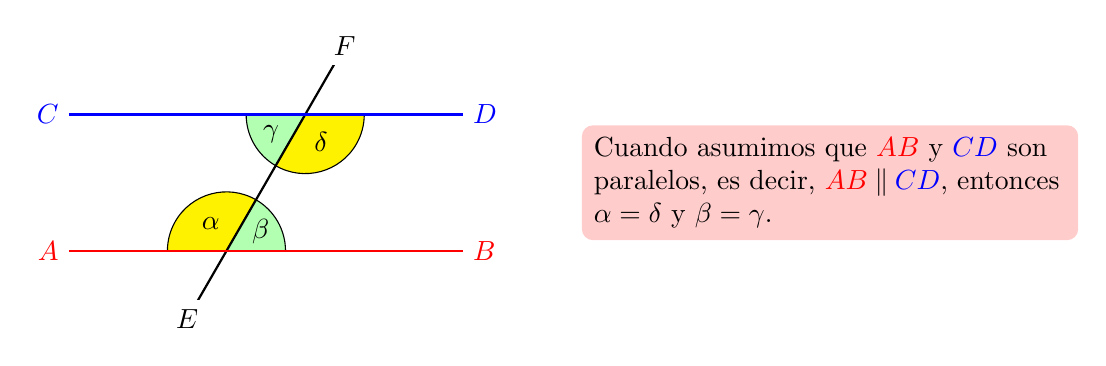
\begin{tikzpicture}
	  \draw[fill=yellow] (0,0) -- (60:.75cm) arc (60:180:.75cm);
	  \draw(120:0.4cm) node {$\alpha$};
	  \draw[fill=green!30] (0,0) -- (right:.75cm) arc (0:60:.75cm);
	  \draw(30:0.5cm) node {$\beta$};
	  \begin{scope}[shift={(60:2cm)}]
	    \draw[fill=green!30] (0,0) -- (180:.75cm) arc (180:240:.75cm);
	    \draw (30:-0.5cm) node {$\gamma$};
	    \draw[fill=yellow] (0,0) -- (240:.75cm) arc (240:360:.75cm);
	    \draw (-60:0.4cm) node {$\delta$};
	  \end{scope}
	  \begin{scope}[thick]
	    \draw  (60:-1cm) node[fill=white] {$E$} -- (60:3cm) node[fill=white] {$F$};
	    \draw[red]                   (-2,0) node[left] {$A$} -- (3,0) node[right]{$B$};
	    \draw[blue,shift={(60:2cm)}] (-3,0) node[left] {$C$} -- (2,0) node[right]{$D$};
	    \draw[shift={(60:1cm)},xshift=4cm]
	    node [right,text width=6cm,rounded corners,fill=red!20,inner sep=1ex]
	    {
	      Cuando asumimos que $\color{red}AB$ y $\color{blue}CD$ son paralelos, es decir, ${\color{red}AB} \mathbin{\|} \color{blue}CD$, entonces $\alpha = \delta$ y $\beta = \gamma$.
	    };
	  \end{scope}
	\end{tikzpicture}
\caption[Ejemplo de uso de PGF/Ti\textit{k}Z]{Ejemplo de uso de PGF/Ti\textit{k}Z, pero solo una muestra de sus capacidades.}
\label{F:tikz}
\end{figure}

Una buena cantidad de ejemplos están disponibles en \url{http://www.texample.net/tikz/} y la documentación (incluyendo un manual de uso de más de 700 páginas) está en \url{https://www.ctan.org/pkg/pgf?lang=en}.

%---------------------------------------
\subsection{Gráfico de datos y funciones con \texttt{pgfplots}}

%---------------------------------------
\subsection{Circuitos con Circuitikz}

El paquete \texttt{circuitikz} permite la creación de circuitos eléctricos y electrónicos. La Figura \ref{F:ampop} es un ejemplo.

\begin{figure}
  	\centering
		 \begin{circuitikz}[american]
		  \draw
		  % El amplificador operacional
		  (0,0) node[op amp] (opamp) {} node[] {{\tiny Amp Op}}
		  
		  % Las entradas
		  (opamp.-) node[circ] {} to[R, l_=$R_1$] ++(-2,0) node[ocirc] {} node[left] {$V_{s}$}
		  (opamp.+) -- ++(0,-0.5) node[ground] {} 
		  
		  % El lazo de realimentación
		  (opamp.-) -- ++(0,1)  to[R, l=$R_2$] ++(2,0) -| (opamp.out) {}
		  
		  % La salida
		  (opamp.out) -- ++(0.5,0) node[circ] {} to[R, l=$R_L$] ++(0,-2) to [short, i_=$I_o$] ++(0,0) node[ground] {}
		  (opamp.out) -- ++(1,0) node[ocirc] {} node[right]{$V_o$}
		  
		  ;
		\end{circuitikz}
    \caption[Amplificador inversor]{Amplificador inversor con un amplificador operacional cuya relación entrada--salida está dada por $V_o = -\frac{R_2}{R_1} V_s$.}
    \label{F:ampop}
\end{figure}

\begin{figure}
\centering
\begin{circuitikz}
\draw
	(0,0)
    	to [V, l=50~\si{\volt}] (0,2) to (0,3)
        to [R, l=$20~\si{\kilo\ohm}$] (5,3) to (5,2)
        to [vR, l=$R$] (5,0)
        to (0,0)
  	(0,2)
    	to [R, l_=$5~\si{\kilo\ohm}$] (5,2)     
;
\end{circuitikz}
\caption{Circuito básico.}
\label{F:circuitobasico}
\end{figure}

\begin{figure}
\centering
\begin{circuitikz}
\draw
	(0,0) node[ground]{}
    	to [V, l=(``Arenal'') $V_{1}$] (0,3)
        to [short] (0.5,3) node[circ]{}
   	(5.5,3)
        to [short] (5.5,4)
        to [R, l=$R_{1}$, i<=$I_{1}$] (3,4)
        to [cV, l=$v_{1}$] (0.5,4)
        to [short] (0.5,3)   
   	(6,3)
    	to [short] (5.5,3)
        to [short] (5.5,2)
        to [R, l=$R_{3}$, i<=$I_{2}$] (3,2)
        to [cV, l=$v_{3}$] (0.5,2)
        to [short] (0.5,3)
	(6,3) node[circ]{}
    	to [generic, i_=$I_{L}$, v^=$v_{L}$] (6,0) node[ground]{}
   	(6,3)
    	to [R, l=$R_{2}$, i<=$I_{3}$] (8.5,3)
        to [cV, l=$v_{2}$] (11,3)
    (11,0) node[ground]{}
        to [V, l_=$V_{2}$ (``Miravalles'')] (11,3)
;
\end{circuitikz}
\caption[Circuito de transmisión de potencia]{Circuito de transmisión de potencia por varias líneas conductoras desde centros de generación y con sistemas de ajuste de la corriente.}
\label{F:transmisionpotencia}
\end{figure}

\begin{figure}
\centering
\begin{circuitikz}
\draw 
(0,0)	to [battery, l_=$V_i$] (0,3)
		to [R, l_=$R_1$] (2.5,3)
        to [cV, l_=$A v_x$] (5,3)
        to [short] (6,3)
        to [vR, l_=$R_T$, i=$i_{R_T}$] (6,0) node[ground]{}
        to [short] (0,0)
(6,3)	to [short] (7,3)
(6,0)	to [short] (7,0)

;
\draw (2.5,3) to [open, v=$v_x$] (2.5,0);
\draw (2.5,3) node[circ]{};
\draw (2.5,0) node[circ]{};

\draw[dashed] (-0.8,-0.8) rectangle (4.8,3.8);
\draw (-0.8,-0.8) node [above right]{Fuente de corriente};

\draw (7,-0.5) rectangle (9,3.5);
\draw (8,1.5) node [align=center]{Circuito \\ de acople};

\draw 
(9,3)	to [short] (10,3)
		to [R, l_=$R_2$] (12,3)
		to [generic, l_=$Y$, v^=$v_Y$] (14,3)
(9,0)   to [short] (14,0) node[ground]{}
		to [cV, l=$A v_z$] (14,3)
(14,0)	to [short] (15.3,0)
		to [open, v>=$v_o$] (15.3,3)
		to [short] (14,3)
;
\draw (12,3)	to [open, v=$v_z$] (12,0);
\draw (12,3) node[circ]{};
\draw (12,0) node[circ]{};

\draw[dashed] (9.8,-0.8) rectangle (14.8,3.8);
\draw (9.8,-0.8) node [above right]{Amplificador};

\draw (15.3,3) node[circ]{} node[right]{$a$};
\draw (15.3,0) node[circ]{} node[right]{$b$};
\end{circuitikz}
\caption[Circuito de acondicionamiento y amplificación]{Circuito de acondicionamiento y amplificación de la señal de un sensor resistivo $R_T$, dependiente de la temperatura.}
\label{F:acondicionamiento}
\end{figure}

\begin{figure}
\centering
\begin{circuitikz}

% PNP Q1
\draw
	(0,4) 	node[pnp,rotate=90](Q1){} node[above]{$Q_1$}
;
% NPN Q2
\draw
	(0,1.5) 	node[npn,rotate=180,yscale=-1](Q2){} node[left]{$Q_2$}
;
% Op Amp
\draw
	(3,1.5) 	node[op amp,rotate=180,yscale=-1](CMP){} node[]{AMP}
;
% Resistores
\draw
	(6,4) node[circ]{} 
    	to [R, l=$R_1$] (6,2) 
    	to [R, l=$R_2$] (6,0) node[ground]{}
;
% Conectores
\draw
	(-1.5,4) 	node[ocirc]{} node[above]{$V_{IN}$} 
    		to [short] (Q1.emitter)
  	(Q1.base) to [short] (Q2.collector)
    (Q2.emitter) to [short] (0,0) node[ground]{}
    (CMP.out) to [short] (Q2.base)
    (Q1.collector) to [short] (7,4) node[ocirc]{} node[above]{$V_{OUT}$}
    (CMP.-) to [short] (6,2) node[circ]{}
    (4.5,0) node[ground]{} to [battery,l_=$V_{R}$] (4.5,1) to [short] (CMP.+) 
;
\end{circuitikz}
\caption{Regulador lineal de tensión con lazo de control.}
\label{F:reguladorlineal}
\end{figure}

\begin{figure}
\centering
\begin{circuitikz} 
\draw
	(0,0) node[op amp,yscale=-1] (opamp) {}
    (0,0) node[](){CMP}
;

\draw 
	(-4.5,2) node[rground, yscale=-1](){} 
    to [I, l_=$I$] (-4.5,1)
    to [short,-*] (-4.5,0.5)
    to [short] (-4.5,-1.8) 
;

\draw 
	(-3,2) node[rground, yscale=-1](){} 
    to [I, l_=$I$] (-3,1)
    to [short,-*] (-3,-0.5) 
    to [R, l_=$R_1$] (-3,-2.5)
    to [R, l_=$R_2$] (-3,-4.5) node[ground](){}
;

\draw 
	(-3,-2.5) to [short,*-] (-2,-2.5)
    to [cspst,] (-2,-4.5) 
    to [short] (-3,-4.5)
    (-1.8,-3.8) node[right](){SW}
;

\draw 
	(-4.5,-2.5) node[pnp](pnp){}
	(pnp.base) node[anchor=east] {\tiny{B}}
    to [short] (-5.3,-4.5) to [short,-*] (-4.5,-4.5)
    (pnp.emitter) node[anchor=east]{\tiny{E}} 
    (pnp.collector) node[anchor=east] {\tiny{C}}
    to [short] (-4.5,-4.5) to [short,-*] (-3,-4.5)
    (-4.5,-2.5) node[anchor=west] {$Q_T$}
;

\draw (opamp.-) to [short] (-3,-0.5) node[anchor=east]{$V^-$};
\draw (opamp.+) to [short] (-4.5,0.5) node[anchor=east]{$V^+$};
\draw (opamp.out) to [short] (1.5,0);
\draw[dashed] (1.5,0) -- (1.5,-3.4) -- (-1.7,-3.4);

\draw (4,0)  node[ocirc]{} node[anchor=south]{\={S}} to [full diode] (1.5,0) node[circ]{} node[anchor=south]{$V_{\mathrm{CMP}}$};

\end{circuitikz}
\caption{Circuito para protección térmica con lazo de histéresis.}
\label{F:protecciontermica}
\end{figure}

\subsection{Inserción de código fuente}
%%%%%%%%%%%%%%%%%%%%%%%%%%%%%%%%%%%%%%%

En ocasiones es necesario introducir secciones de código fuente de programación dentro de reportes. La inserción es especial, pues el compilador no debe confundir las instrucciones dentro del código con instrucciones de \LaTeX. Además, se prefiere un formato específico con resaltado de sintaxis para mejorar la legibilidad (como en los editores de código o en los IDE). Un paquete que provee soluciones para este requisito es \texttt{listings}.

Para el código fuente hecho en Matlab es posible utilizar el paquete \texttt{mcode} (adjunto como archivo a la carpeta que contiene el proyecto) que asigna a \texttt{listings} el formato apropiado, como se ve en el siguiente código:

\lstinputlisting[inputencoding=latin1]{codigo/codigoejemplo.m}

%%%%%%%%%%%%%%%%%%%%%%%%%%%%%%%%%
\section{Referencias para \LaTeX}
%%%%%%%%%%%%%%%%%%%%%%%%%%%%%%%%%

La comunidad de usuarios de \LaTeX~ es grande y colaborativa. Hay multitud de recursos en línea para aprender buenas prácticas y ``trucos'' para mejorar los documentos. Algunas de las mejores referencias son:

\begin{description}
\item[Wikibook] \url{https://en.wikibooks.org/wiki/LaTeX}
\item[Cookbook] \url{http://latex-cookbook.net/}
\item[TeXample] \url{http://texample.net/}
\item[HowtoTeX] \url{http://www.howtotex.com/}
\item[Font Catalogue] \url{http://www.tug.dk/FontCatalogue/}
\end{description}

\subsection{¿Dónde editar \LaTeX?}\label{S:programas}
%%%%%%%%%%%%%%%%%%%%%%%%%%%%%%%%%%%%%%%%%%%

\paragraph{Editores de texto ``de escritorio''}

Existen varios programas para la edición y compilación de archivos de \LaTeX. Se ha escogido Texmaker debido a que es multiplataforma (Mac, Linux, Windows) y cuenta con otras características como resaltado de sintaxis, autocompletar, corrección ortográfica, asistente para la creación de documentos, accesos rápidos a símbolos, comandos y entornos, entre otros. Se puede, claro está, editar el documento con cualquier editor y compilar, siempre y cuando se tengan los paquetes necesarios\footnote{Esta es una ventaja de ser un código estándar abierto.}.

En Windows, junto con Texmaker debe instalarse MiKTeX, que es un conjunto de paquetes, fuentes y demás necesarios para compilar el archivo.

Ambos están disponibles para descarga gratuita desde \url{http://miktex.org/} y \url{http://www.xm1math.net/texmaker/}.

Una base de datos extensiva de los paquetes de \LaTeX~ está en \url{http://www.ctan.org/}. Es especialmente útil para encontrar la documentación de los paquetes. Desde esta página se pueden descargar los paquetes, pero la mejor forma de revisar los paquetes disponibles e instalarlos fácilmente es a través del \emph{MiKTeX Package Manager}, disponible después de instalar el MiKTeX.

\paragraph{Plataformas en línea de edición para \LaTeX}

Una alternativa muy popular de años muy recientes es la edición en línea. Entre las ventajas se encuentran: almacenamiento en línea, edición colaborativa, herramientas web (bibliografías y otros), compilación simultánea, más la mayoría de las otras ventajas de los editores ``de escritorio'' como autocompletar, símbolos, etc.

Los editores más populares son:

\begin{description}
\item[Overleaf] \url{https://www.overleaf.com/}
\item[ShareLaTeX] \url{https://www.sharelatex.com/}
\item[Papeeria] \url{https://papeeria.com/}
\end{description}
%% ----------------------------------------
  \chapter{Conclusiones y recomendaciones}
% ----------------------------------------
\label{C:conclusiones}

El informe debe terminarse con la enumeración de las principales conclusiones derivados del trabajo realizado.  En particular, debe verificarse el cumplimiento de los objetivos planteados para el mismo.

\section{Conclusiones}
El aporte (\emph{novedad}) hecho con el proyecto, debe destacarse.

Las conclusiones pueden enumerarse en forma suscinta como una lista, ya sea itemizada o numerada.

\section{Recomendaciones}
Con base en las trabajo realizado y las conclusiones sobre el mismo, puede ser necesario incluir una sección, o lista, de recomendaciones.  Por ejemplo, sobre la utilización de otro enfoque para resolver el problema.

% 9. APÉNDICES
% ------------
\appendix
\chapter{Actobotics 638276}

A continuación, la siguiente página muestra las especificaciones del fabricante de los motores DC Actobotics utilizados en el proyecto.

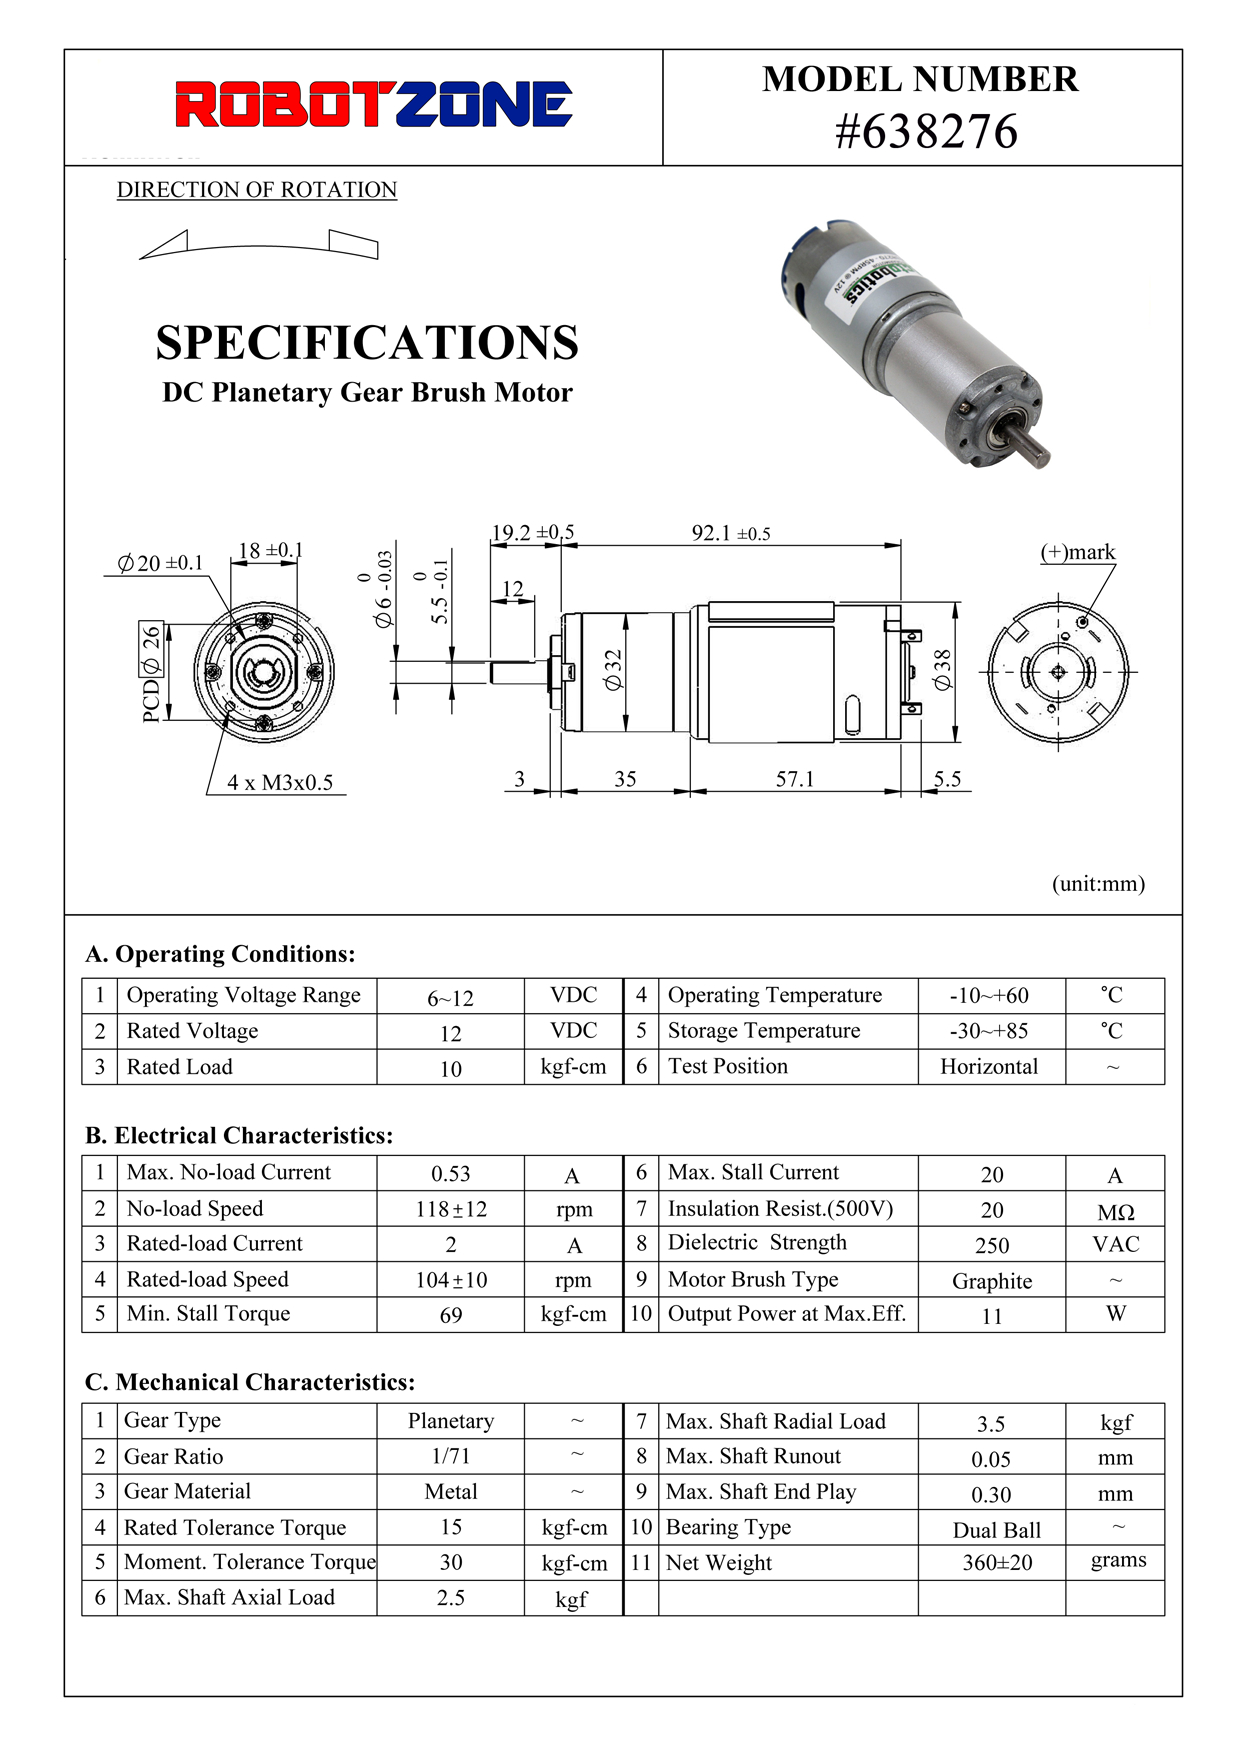
\includepdf[pages=1]{fabricante/servomotor.pdf}


%%% Local Variables:
%%% mode: latex
%%% TeX-master: t
%%% End:

\chapter{STM32F4 Encoder}

A continuación, las siguientes tres páginas representan la información contenida en el manual de usuario del stm32f411 con respecto a el funcionamiento de los encoders de cuadratura, y la configuración pertinente del lado del stm.

\includepdf[pages=277-279]{fabricante/rm0383.pdf}
%%% Local Variables:
%%% mode: latex
%%% TeX-master: t
%%% End:

\chapter{Roboclaw Instrucciones}

A continucación se muestran tres páginas con información relevante para la escritura de una librería de comunicación hacia el controlador de motores Roboclaw.

\includepdf[pages={64-65,70}]{fabricante/roboclaw_user_manual.pdf}

%%% Local Variables:
%%% mode: latex
%%% TeX-master: t
%%% End:

\backmatter

% 10. BILIOGRAFÍA
% --------------
\bibliographystyle{plain}
\bibliography{contenido/bibliografia.bib}

%%%%%%%%%%%%%%%%%%%
\end{document}
%%%%%%%%%%%%%%%%%%%
